\subsection{Orthogonalized State Update}

\noindent
In sequence modeling for echocardiography video segmentation, preserving spatial details (\eg,~rapid valvular motion and subtle myocardial deformations) across long sequences is essential.
Standard linear recurrent models \cite{katharopoulos_transformers_2020,ICML20_ttt,ICML21_fwp,ICLR25_gdn,ICLR26_ttt_LaCT} encode historical information into a hidden state $\mathbf{S}_t \in \mathbb{R}^{C_v \times C_k}$, where we assume $C_v \ge C_k$.

The gated recurrent update \cite{ICLR25_gdn,ICCV25_gdkvm,arxiv25_kimidelta} corresponds to a proximal gradient descent step in unconstrained Euclidean space~\cite{FTO16_Hazan}.
At each timestep $t$, the incoming data introduces a linearized surrogate objective $\ell_t(\mathbf{S}) = -\operatorname{Tr}(\mathbf{G}_t^\top \mathbf{S})$, where $\mathbf{G}_t = \beta_t (\mathbf{v}_t - \alpha_t \mathbf{S}_{t-1} \mathbf{k}_t) \mathbf{k}_t^\top$ denotes the gradient.
The unconstrained state evolution minimizes this surrogate, regularized by a Euclidean proximity term:
\begin{equation}
  \begin{aligned}
    \mathbf{S}_t^{\text{Euc}} &= \mathbf{S}_{t-1}\left(\alpha_t (\mathbf{I}_{C_k} - \beta_t \mathbf{k}_t \mathbf{k}_t^\top)\right) + \beta_t \mathbf{v}_t \mathbf{k}_t^\top \\
    &= \underset{\mathbf{S} \in \mathbb{R}^{C_v \times C_k}}{\arg\min} \left( \ell_t(\mathbf{S}) + \frac{1}{2} \|\mathbf{S} - \alpha_t \mathbf{S}_{t-1}\|_F^2 \right).
  \end{aligned}
\end{equation}
However, performing gradient descent directly in unconstrained Euclidean space lacks intrinsic geometric regularization.
The gating mechanism $\alpha_t$ acts as an isotropic shrinkage.
In echocardiography video segmentation, the combination of this unconstrained shrinkage and the successive rank-1 data updates ($\mathbf{k}_t \mathbf{k}_t^\top$) alters the spectrum of the hidden state matrix.
Specifically, dominant update directions are amplified while orthogonal components decay, leading to rank collapse \cite{ICML16_urnn,NIPS16_fullurnn}.

\noindent
\textbf{Orthogonalized state update on the Stiefel manifold.}
To address this rank collapse, we propose \emph{Orthogonalized State Update}, which constrains the state evolution to the Stiefel manifold via an orthogonalized update
\begin{equation}
    \label{eq:stiefel_manifold}
    \mathcal{V}_{C_v, C_k} = \{\mathbf{S} \in \mathbb{R}^{C_v \times C_k} : \mathbf{S}^\top \mathbf{S} = \mathbf{I}_{C_k}\}.
\end{equation}
\begin{equation}
  \mathbf{S}_t = \operatorname{Proj}_{\mathcal{V}}(\mathbf{S}_t^{\text{Euc}}) = \underset{\mathbf{S} \in \mathcal{V}_{C_v, C_k}}{\arg\min} \frac{1}{2} \|\mathbf{S} - \mathbf{S}_t^{\text{Euc}}\|_F^2.
\end{equation}
By enforcing strict orthogonality, the Frobenius norm of the state remains constant ($\|\mathbf{S}_t\|_F^2 = C_k$).
Consequently, the projection is equivalent to maximizing the trace inner product: $\arg\max_{\mathbf{S} \in \mathcal{V}} \operatorname{Tr}(\mathbf{S}^\top \mathbf{S}_t^{\text{Euc}})$, which identifies the closest orthogonal matrix to $\mathbf{S}_t^{\text{Euc}}$.

        \begin{figure}[!t]
    \centering
    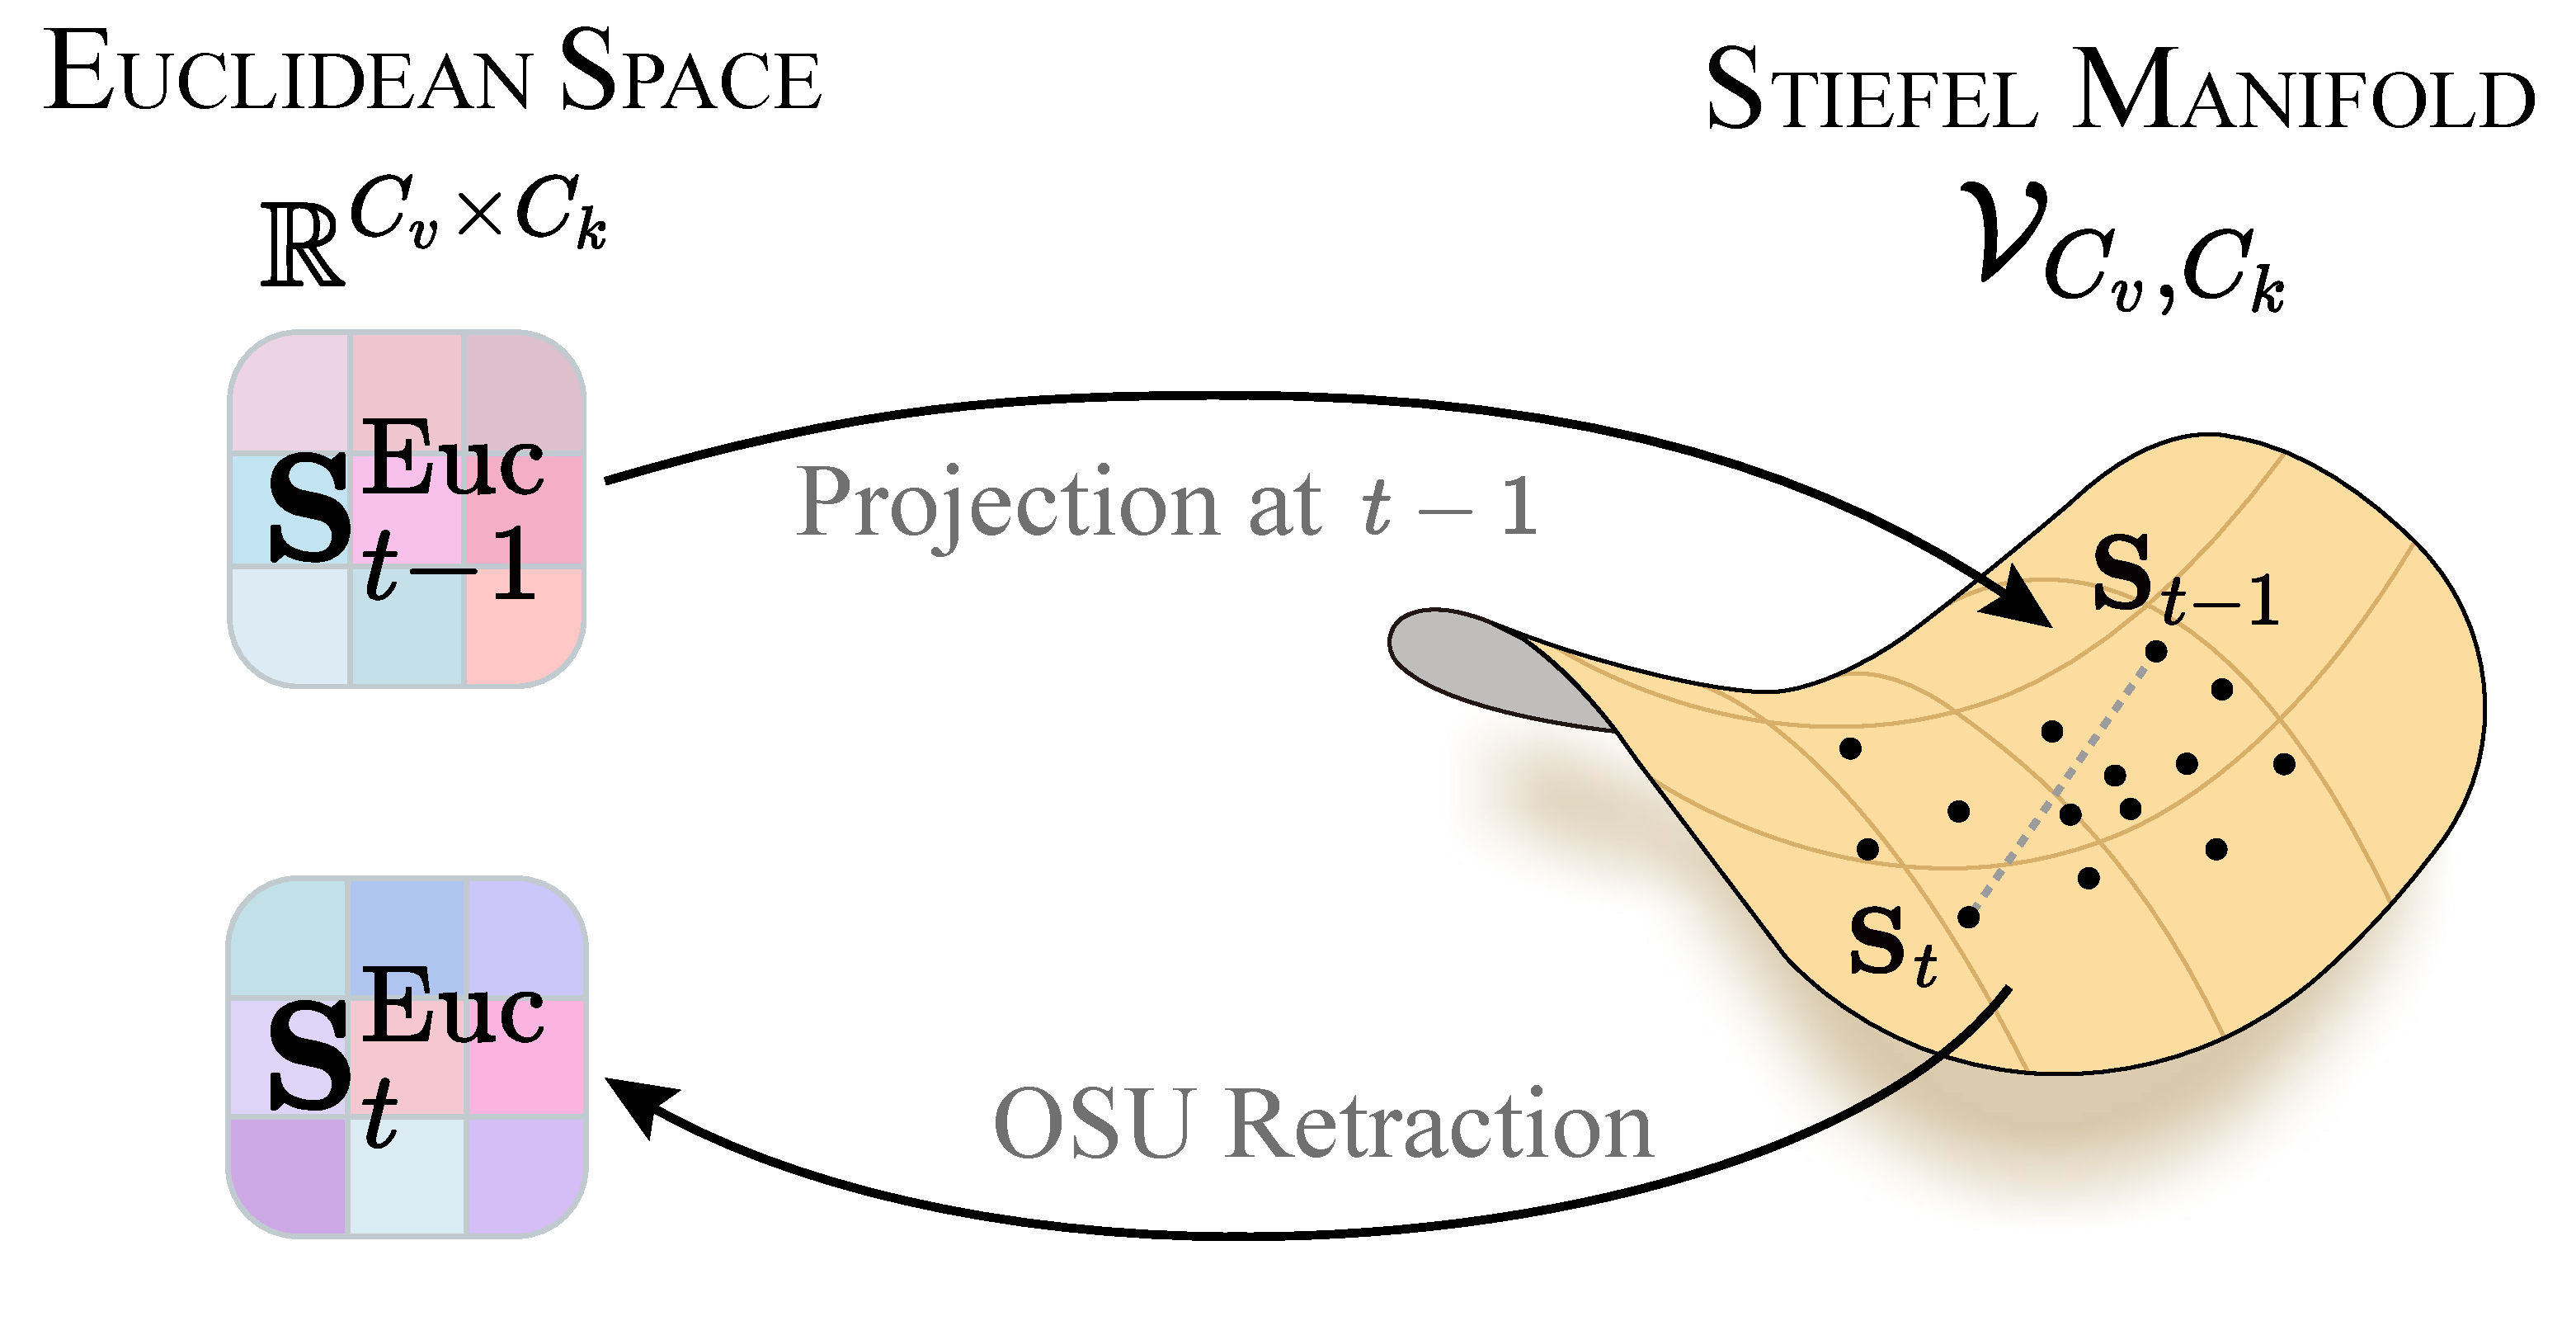
\includegraphics[width=0.94\linewidth]{fig/osu/fig_osu.pdf}
    \caption{Illustration of OSU.
    Standard Euclidean recurrences suffer from rank collapse over long sequences (manifested as singular value decay and increasing condition number). OSU constrains state evolution on the Stiefel manifold via orthogonalized update. The unconstrained intermediate state $\mathbf{S}_t^{\text{Euc}}$ is projected back to the manifold as $\mathbf{S}_t$, ensuring stable temporal transitions.}
    \label{fig:osu}
\end{figure}

\begin{figure}[!t]
    \centering
    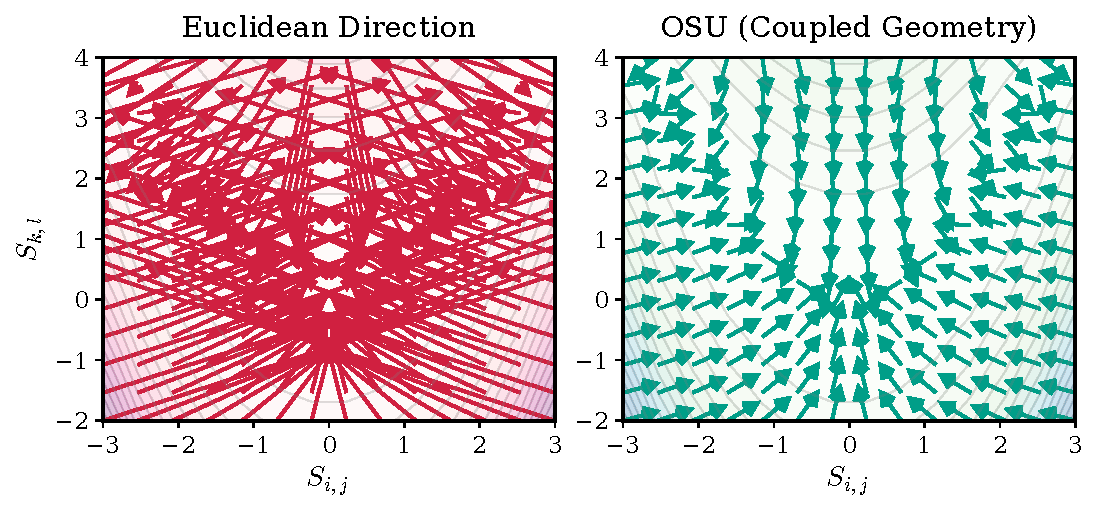
\includegraphics[width=1.0\linewidth]{fig/landscape_2d/fig_landscape_2d.pdf}
    \caption{\textbf{Behavioral comparison of optimization vector fields.}
    Unconstrained Euclidean updates cause the state to drift away from orthogonal constraints (climbing valley walls). OSU generates a corrective flow that pulls iterates back onto the Stiefel manifold (valley floor).}
    \label{fig:landscape_2d_behavior}
\end{figure}

As illustrated in~\cref{fig:osu}, the standard Euclidean recurrence (left) allows the state to deviate from the manifold, whereas OSU explicitly projects $\mathbf{S}_t^{\text{Euc}}$ back onto the Stiefel manifold to preserve orthogonality.
\Cref{fig:landscape_2d_behavior} further visualizes this from an optimization perspective: unconstrained updates deviate from the manifold constraint, while OSU projects the iterates back onto the feasible region.

\noindent
\textbf{High-order Newton-Schulz iteration for efficient projection.}
The exact solution computes the orthogonal polar factor via SVD~\cite{SIAM86_Higham}, incurring $\mathcal{O}(C_v C_k^2)$ cost.
To reduce this computational cost, we employ a parameterized high-order Newton-Schulz iteration \cite{SIAM06_Schur,SIAM06_Newton}, which converges to the closest orthogonal matrix faster than standard quadratic schemes.
Newton-Schulz iterations converge only when the initial singular values are strictly bounded.
Because the Frobenius norm upper-bounds the spectral norm ($\|\cdot\|_2 \le \|\cdot\|_F$), scaling the intermediate unconstrained state by its Frobenius norm provides a sufficient bound to ensure all singular values fall strictly within this convergence domain:
\begin{equation}
  \mathbf{X}^{(0)} = \frac{\mathbf{S}_t^{\text{Euc}}}{\|\mathbf{S}_t^{\text{Euc}}\|_F + \epsilon},
\end{equation}
where $\epsilon$ is a small constant ensuring numerical stability.
The orthogonalization is then performed using a 5th-order polynomial expansion:
\begin{equation}
  \mathbf{X}^{(j+1)} = a\mathbf{X}^{(j)} + b\mathbf{X}^{(j)}{\mathbf{X}^{(j)}}^\top \mathbf{X}^{(j)} + c\mathbf{X}^{(j)}({\mathbf{X}^{(j)}}^\top \mathbf{X}^{(j)})^2.
\end{equation}
The polynomial coefficients $a$, $b$, and $c$ are configured to optimize the spectral mapping function, thereby maximizing the rate of convergence towards the Stiefel manifold.
In practice, this iteration achieves orthogonality in a fixed number of steps, avoiding the exact SVD computation.

This orthogonalization stabilizes the representation spectrum.
In our sequence modeling implementation, projecting onto the Stiefel manifold acts as an effective constant spectral norm constraint ($\|\mathbf{S}_t\|_2 = \gamma$, where $\gamma$ is a non-zero scaling factor applied to the projected state).
By preventing singular value decay and bounding the condition number, our method avoids the rank collapse typically observed in unconstrained recurrent updates.
This scaled isometry maintains norm stability during state transitions, supporting long-range dependency modeling for echocardiography video segmentation by preserving consistent feature representations across complete cardiac cycles.